\chapter{Results and Discussion}

\section{Sequences}
\noindent The first step of our methodology was to study the sequences of the GSTs of interest. We computed their Multiple Sequence Alignment as well as the percent identity matrix associated. This allows to identify regions of high/low conservation as well as group of sequences that are self-similar. For instance, in the figure \ref{Sequence and Structure matricies} it is clearly visible on the pannel A that among the class $\delta$, the GSTs are self similar. In contradiction, it seems that among the class $\varepsilon$, the GSTs E5, E6, E7, E8 are self similar but the other ones seems much more different. This is even more visible in the pannel B where we computed the probability  of identity in the considered set of sequences. The red histogram take into account the whole matrix and it apears that the identity is of $30-40\%$ within almost $60\%$ of the sequences but when we consider only the comparitions between sequences from a given class, we have usually $60-70\%$ of identity for the class $\delta$ and $40-50\%$ for the class $\varepsilon$.

\begin{figure}[H]
	\label{Sequence and Structure matricies}
	\begin{minipage}{.33\linewidth}
		\textbf{A}\\
		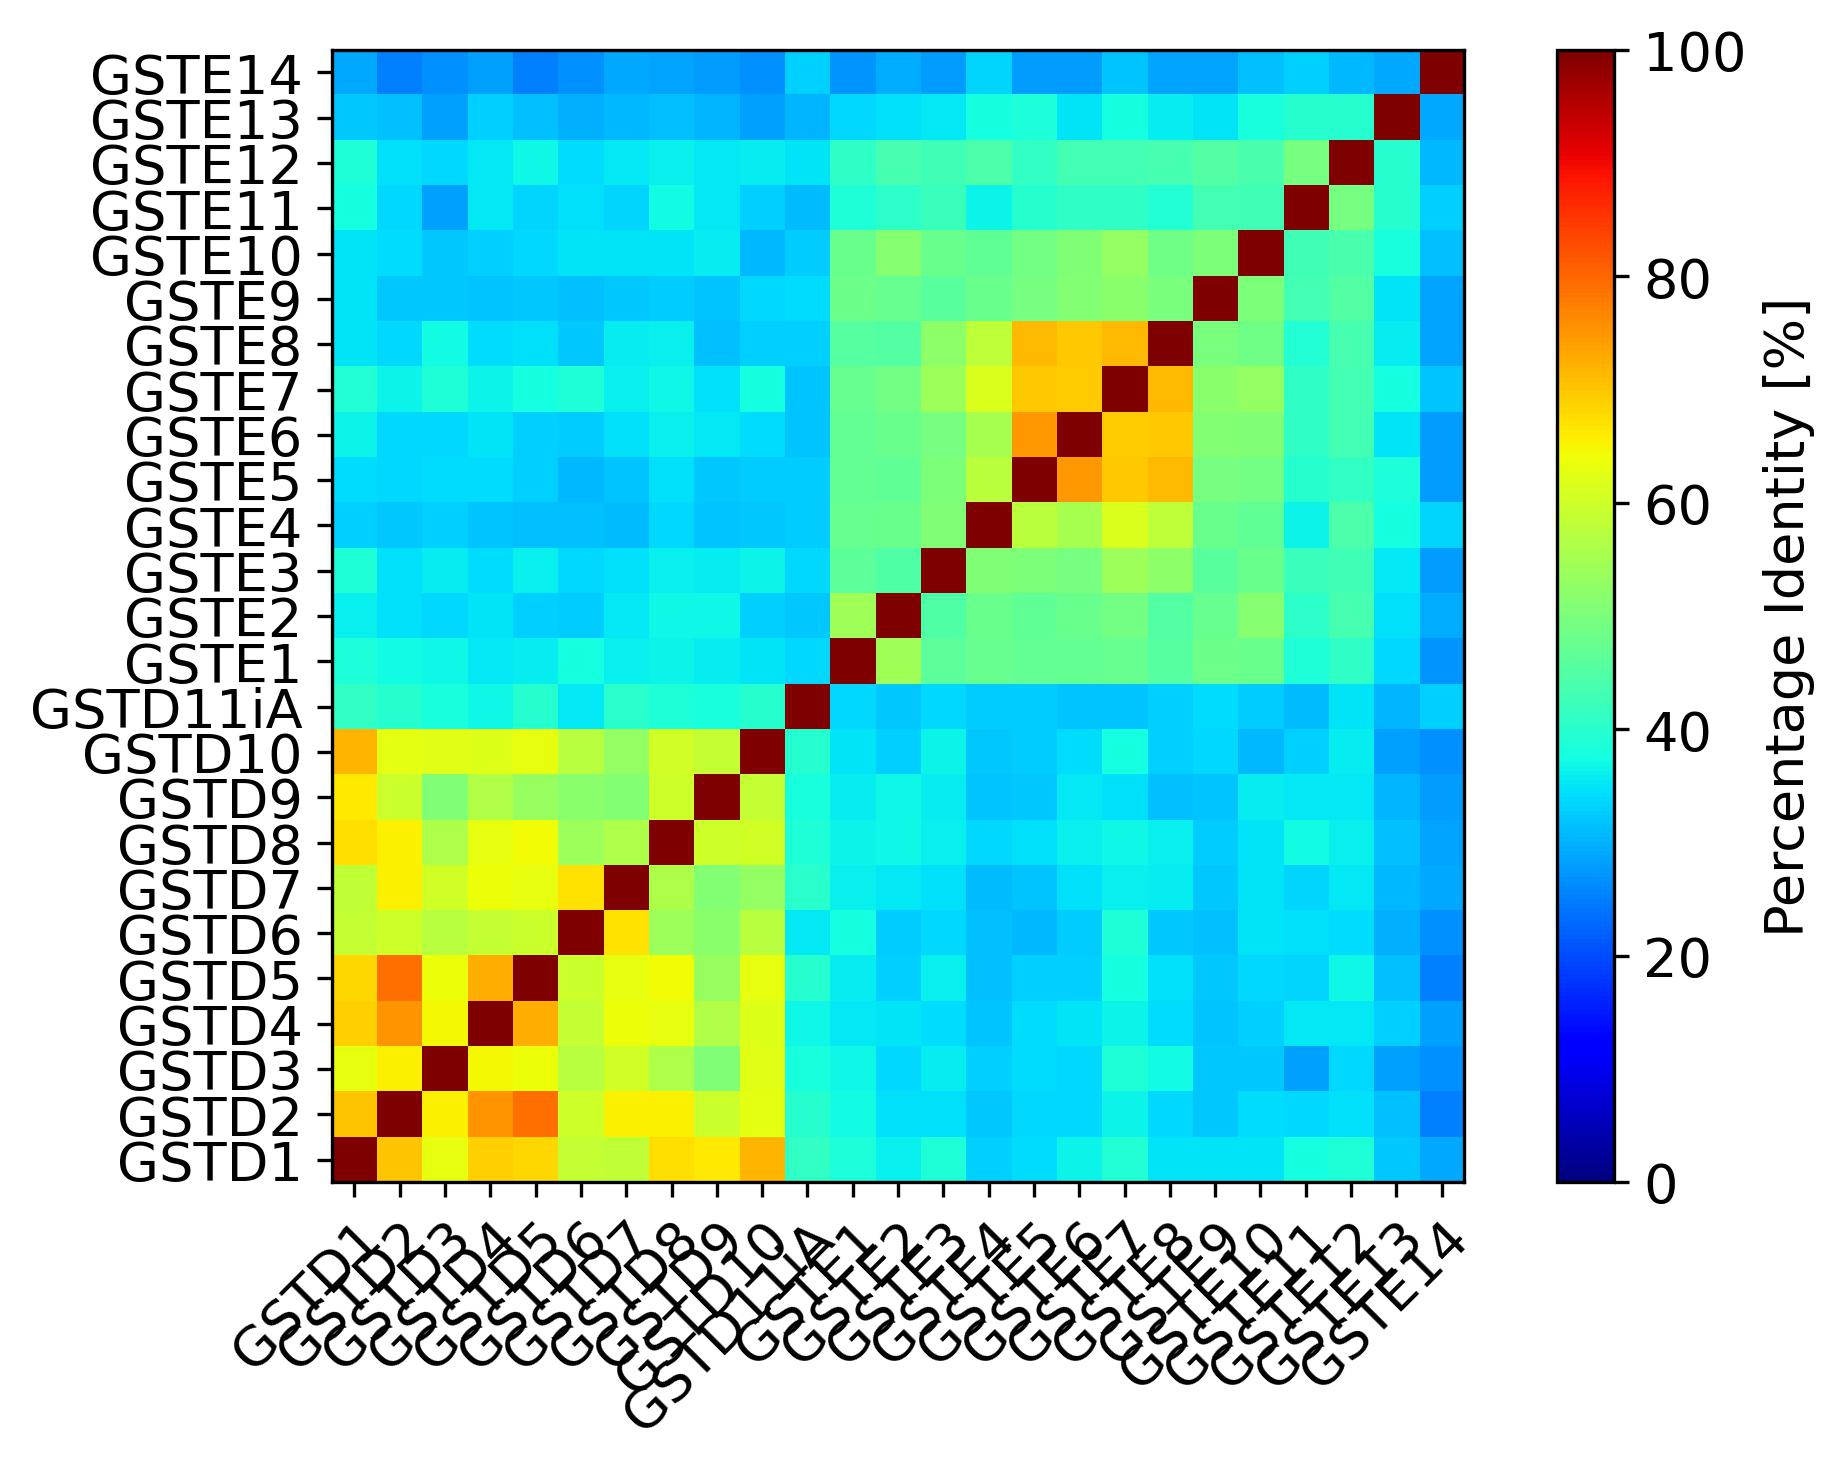
\includegraphics[height = 4cm]{figures/PercentID_matrix.jpg}
	\end{minipage}
	\begin{minipage}{.65\linewidth}
		\textbf{B}\\
		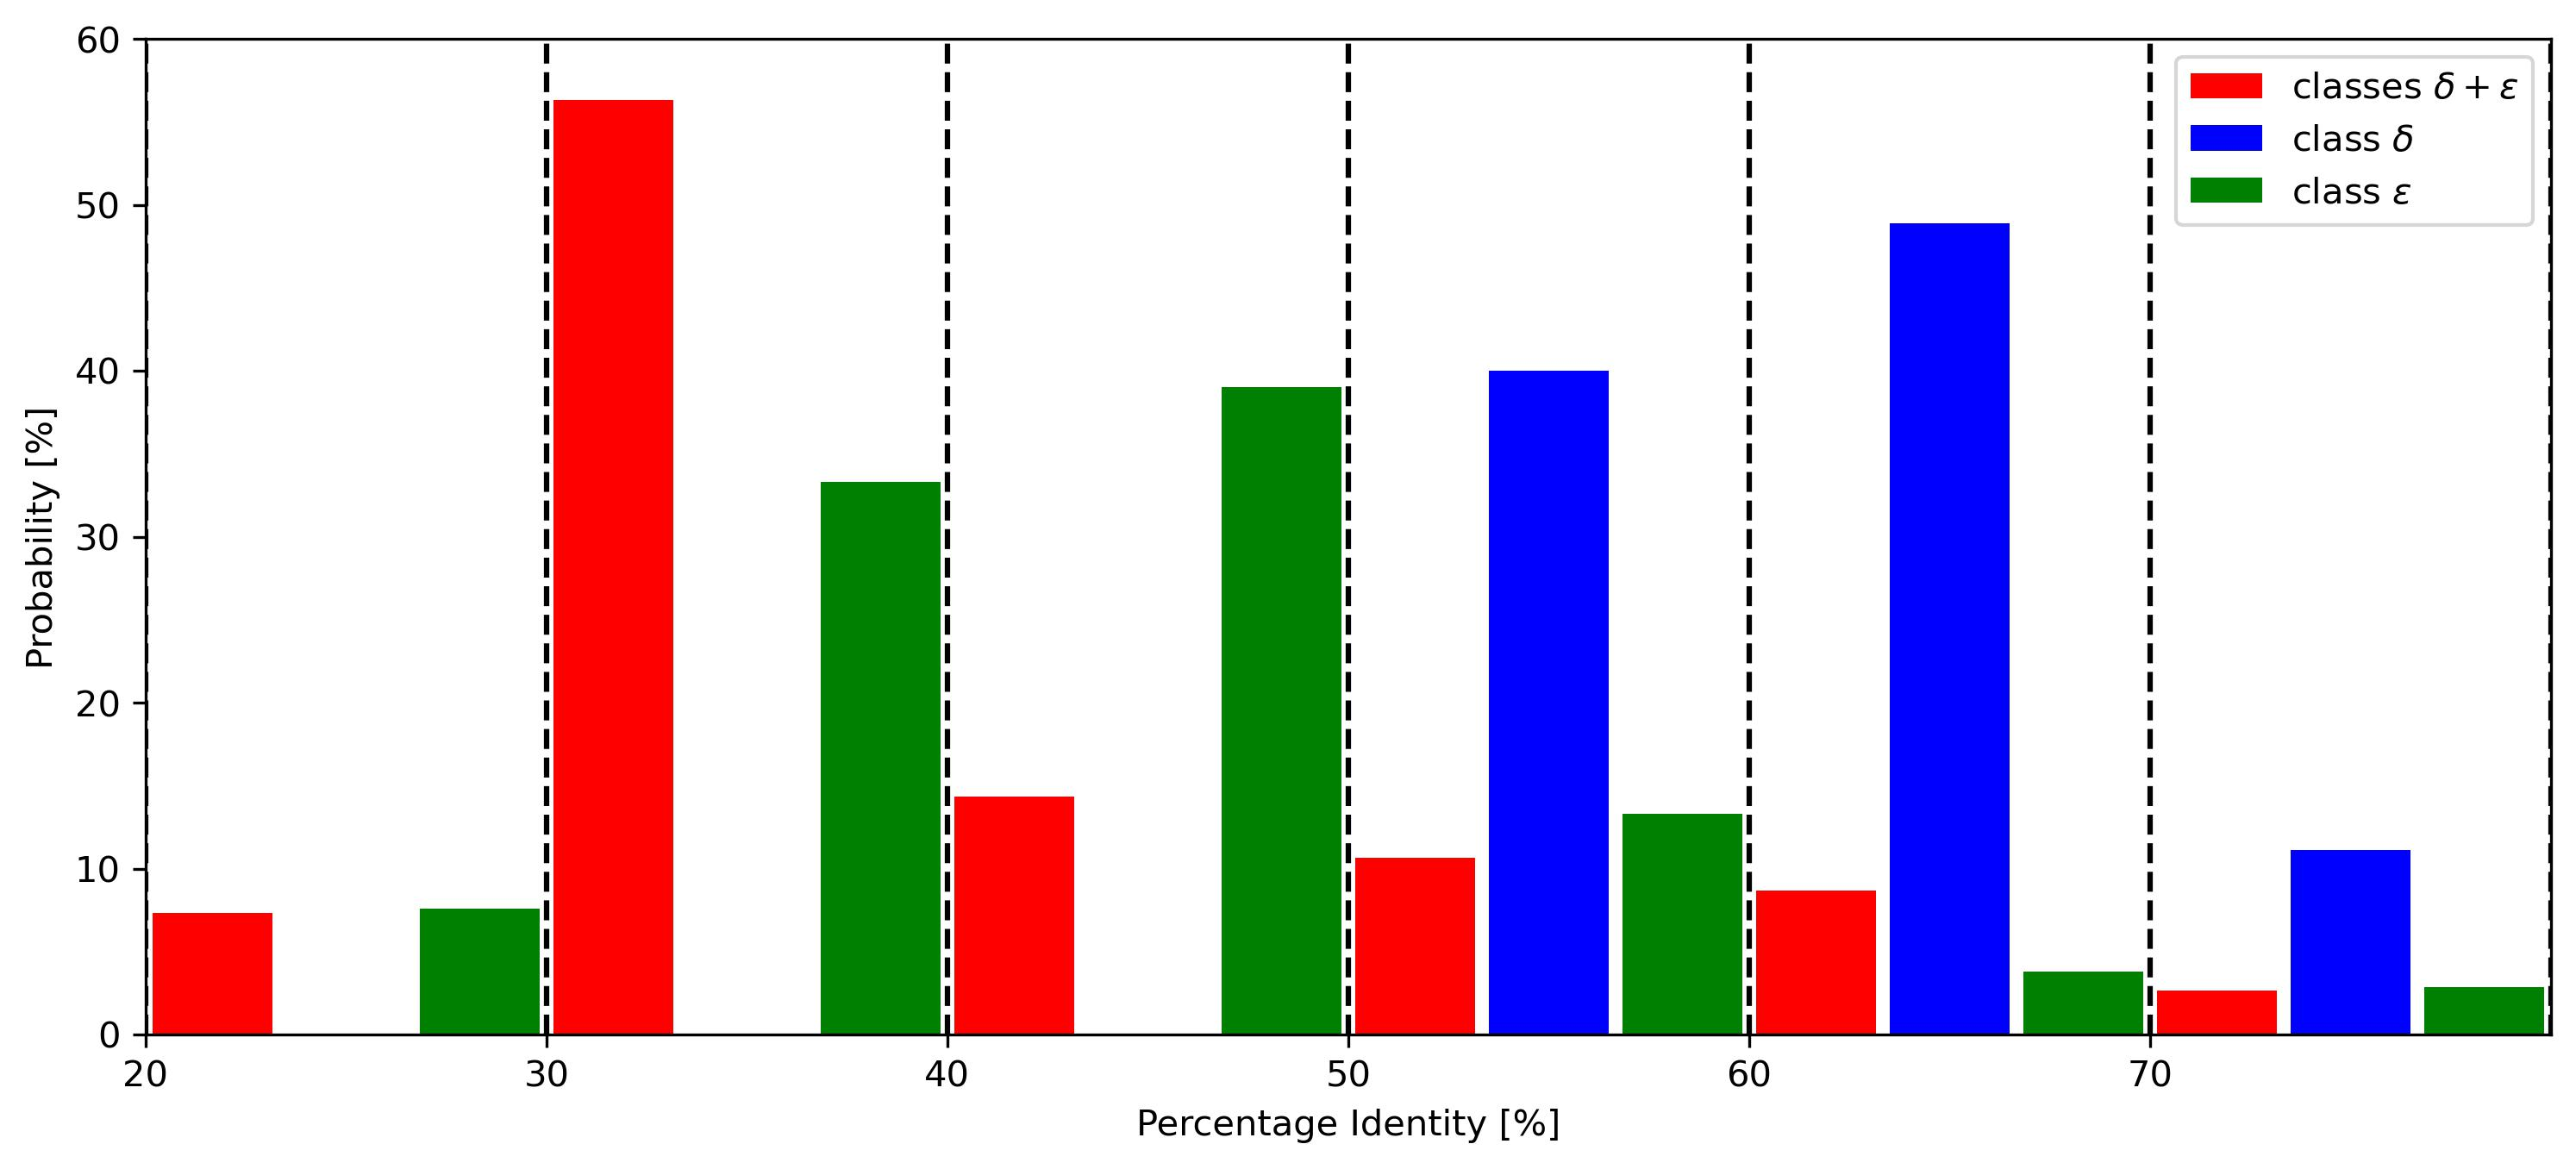
\includegraphics[height = 4cm]{figures/PercentID_proba.jpg}
	\end{minipage}
	\caption{Percent identity matrix and probability from the GST sequences}
\end{figure}

\section{Structures}

\begin{figure}
	\label{AlphaFold structures}
	\includegraphics[width = .99\linewidth]{figures/GSTs_array}
	\caption{GST's structures predicted from AlphaFold}
\end{figure}

The sequences were then used as a base for the AlphaFold program to predict the 3D structure (cf. figure \ref{AlphaFold structures}) and pairs of structures were compared using the Root Mean Squared Deviation (i.e. geometrical distances between atoms, pannel A) and once again in the associated matrix, one can identify two main clusters for class $\delta$ and $\varepsilon$ but here the E10 gives much higher values than we might have expect. This is due to a much longer sequence in the terminal part that make the RMSD higher. Eventually, one can remark that for most of the GSTs in the class $\varepsilon$, the terminal parts have any predicted structures. This is either due to a convergence problem in the AlphaFold predictions or to a biological feature of those proteins that isn't yet well known. 

\begin{figure}[H]
	\label{AlphaFill & GSHs}
	\begin{minipage}{.48\linewidth}
		\textbf{A}\\
		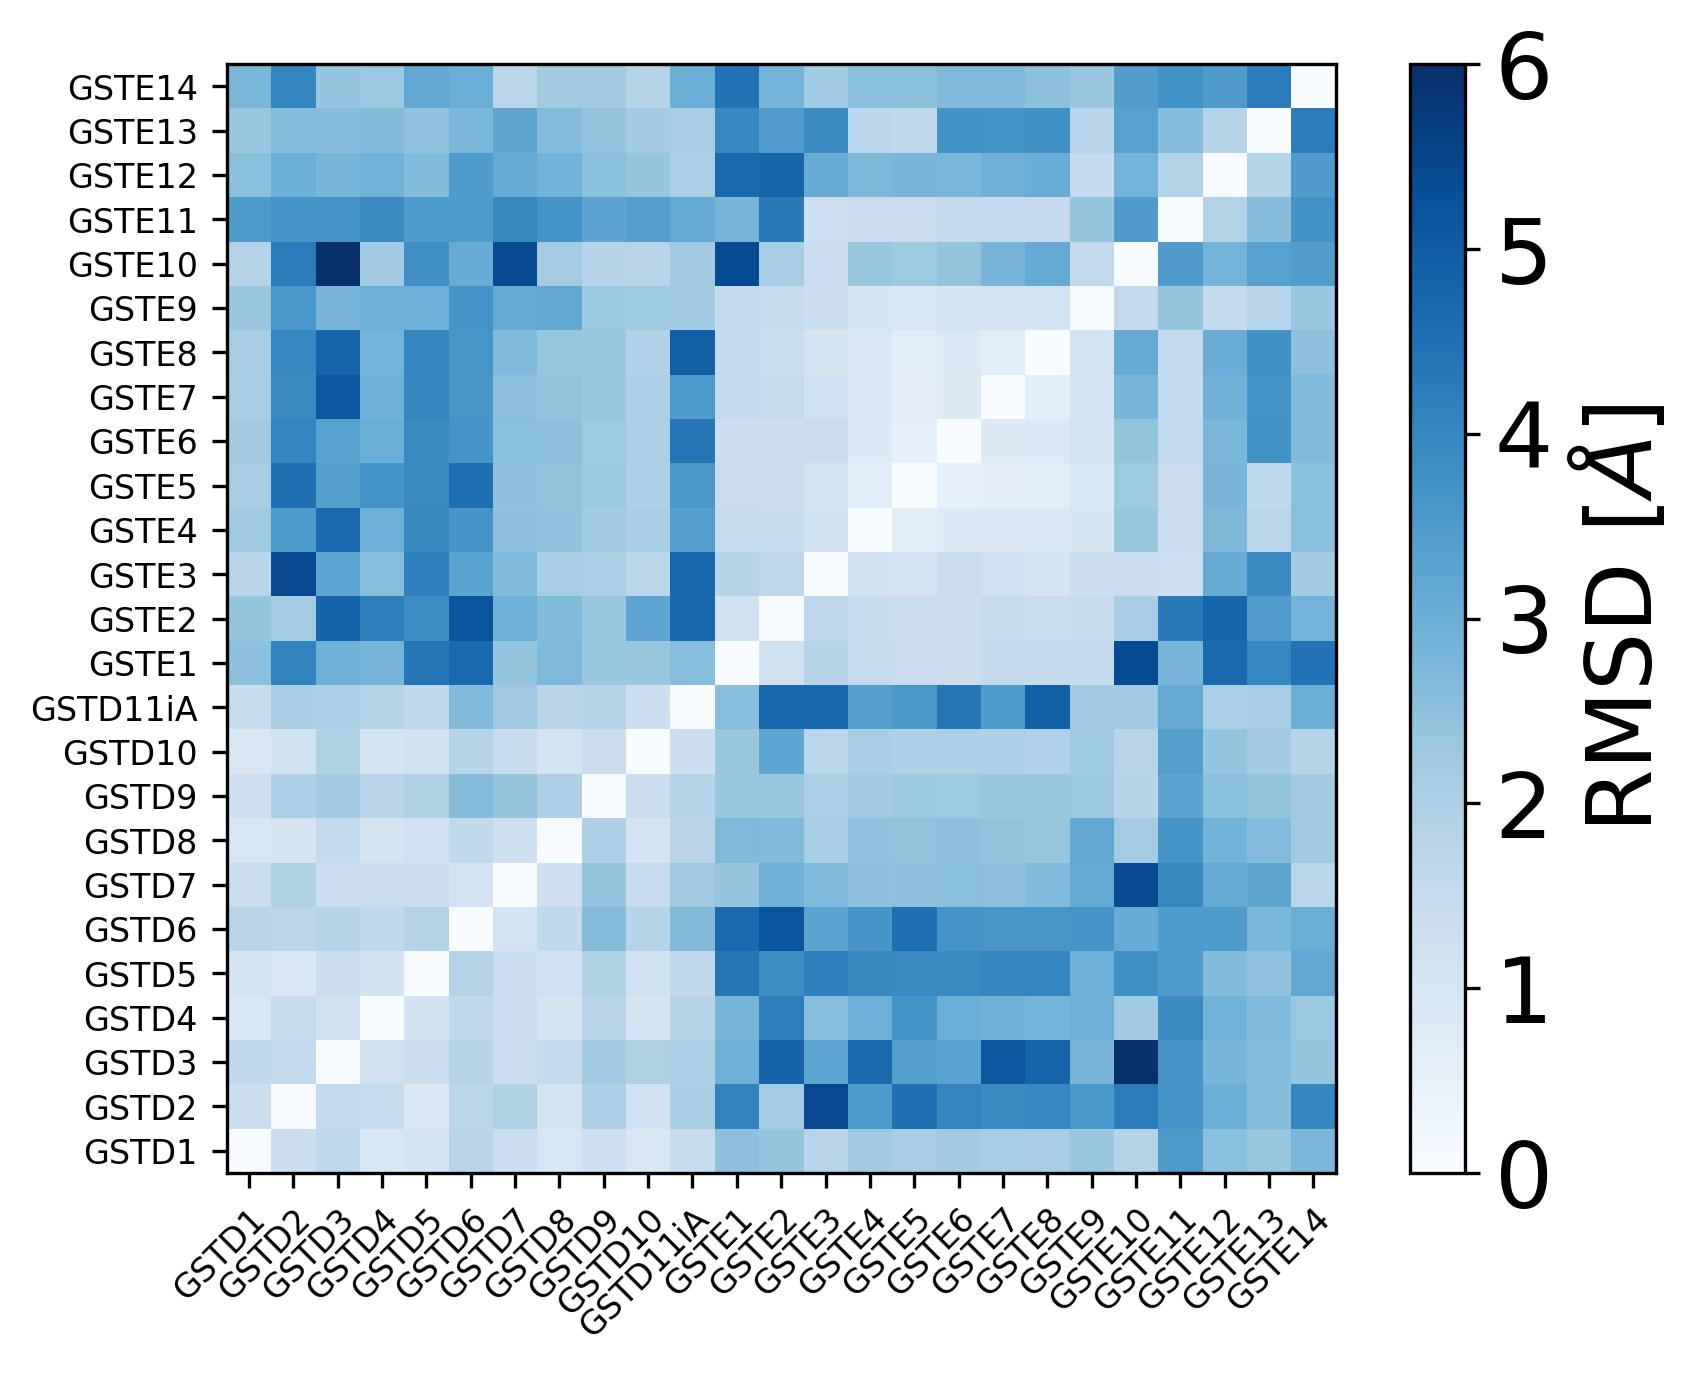
\includegraphics[height = 6cm]{figures/RMSD_matrix.jpg}
	\end{minipage}
	\begin{minipage}{.48\linewidth}
		\textbf{B}\\
		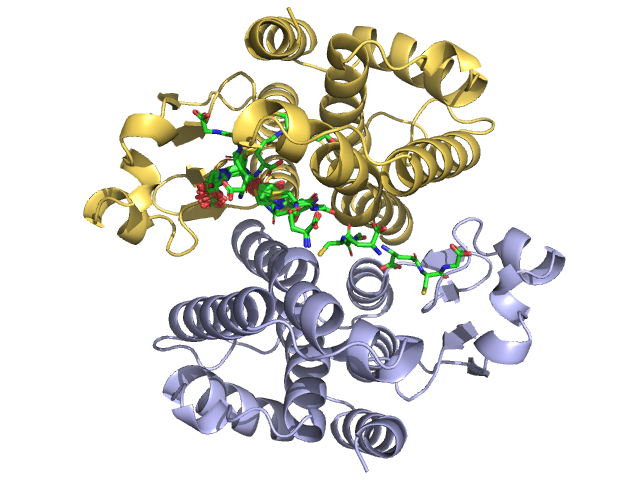
\includegraphics[height = 6cm]{figures/GSTD1_GSHs.png}
	\end{minipage}
	\caption{Geometrical comparitions between AlphaFold predicted structures \& illustration of the predictions of AlphaFill in the case of the GSTD1}
\end{figure}

\section{Conservation}

\noindent From the structures and based on distance matricies between the atoms, it is possible to look at the interface of dimerization (i.e. the residues that are involved in the monomer-monomer binding). We also used this method to determine the Binding site of the ligands. As mantioned earlier, the program AlphaFill allows to make such precisions and this gives $40$ different positions of Glutathion-like ligands in the GSTD1 (i.e. ligands that are chemically close to Glutathione), those positions are represented in the 3D structure (figure \ref{AlphaFill & GSHs} pannel B). Distances between atoms allowed us to determine from these data the residues that are involved in the protein-ligand binding as well as the dimerization of the structure. Indeed, two atoms that are closer than $3$\AA ~were considered as in contact. This information can be computed for all 25 structures and projected on the MSA matrix computed before. This gives the following representation (see Fig. \ref{MSA + AF + AFi}), where we computed the probability of a given residue to be in the binding site or in the interface of dimerization. From this information, we are able to compute the conservation of any residue in the binding site / interface of dimerization. Here, we give an illustration in the case of the residue $124$, which have a high degree of conservation among all the studied GSTs and have been identified as a part of the binding site in $\%$.

\begin{figure}
	\label{MSA + AF + AFi}
	\raggedright\textbf{A}\\
	\center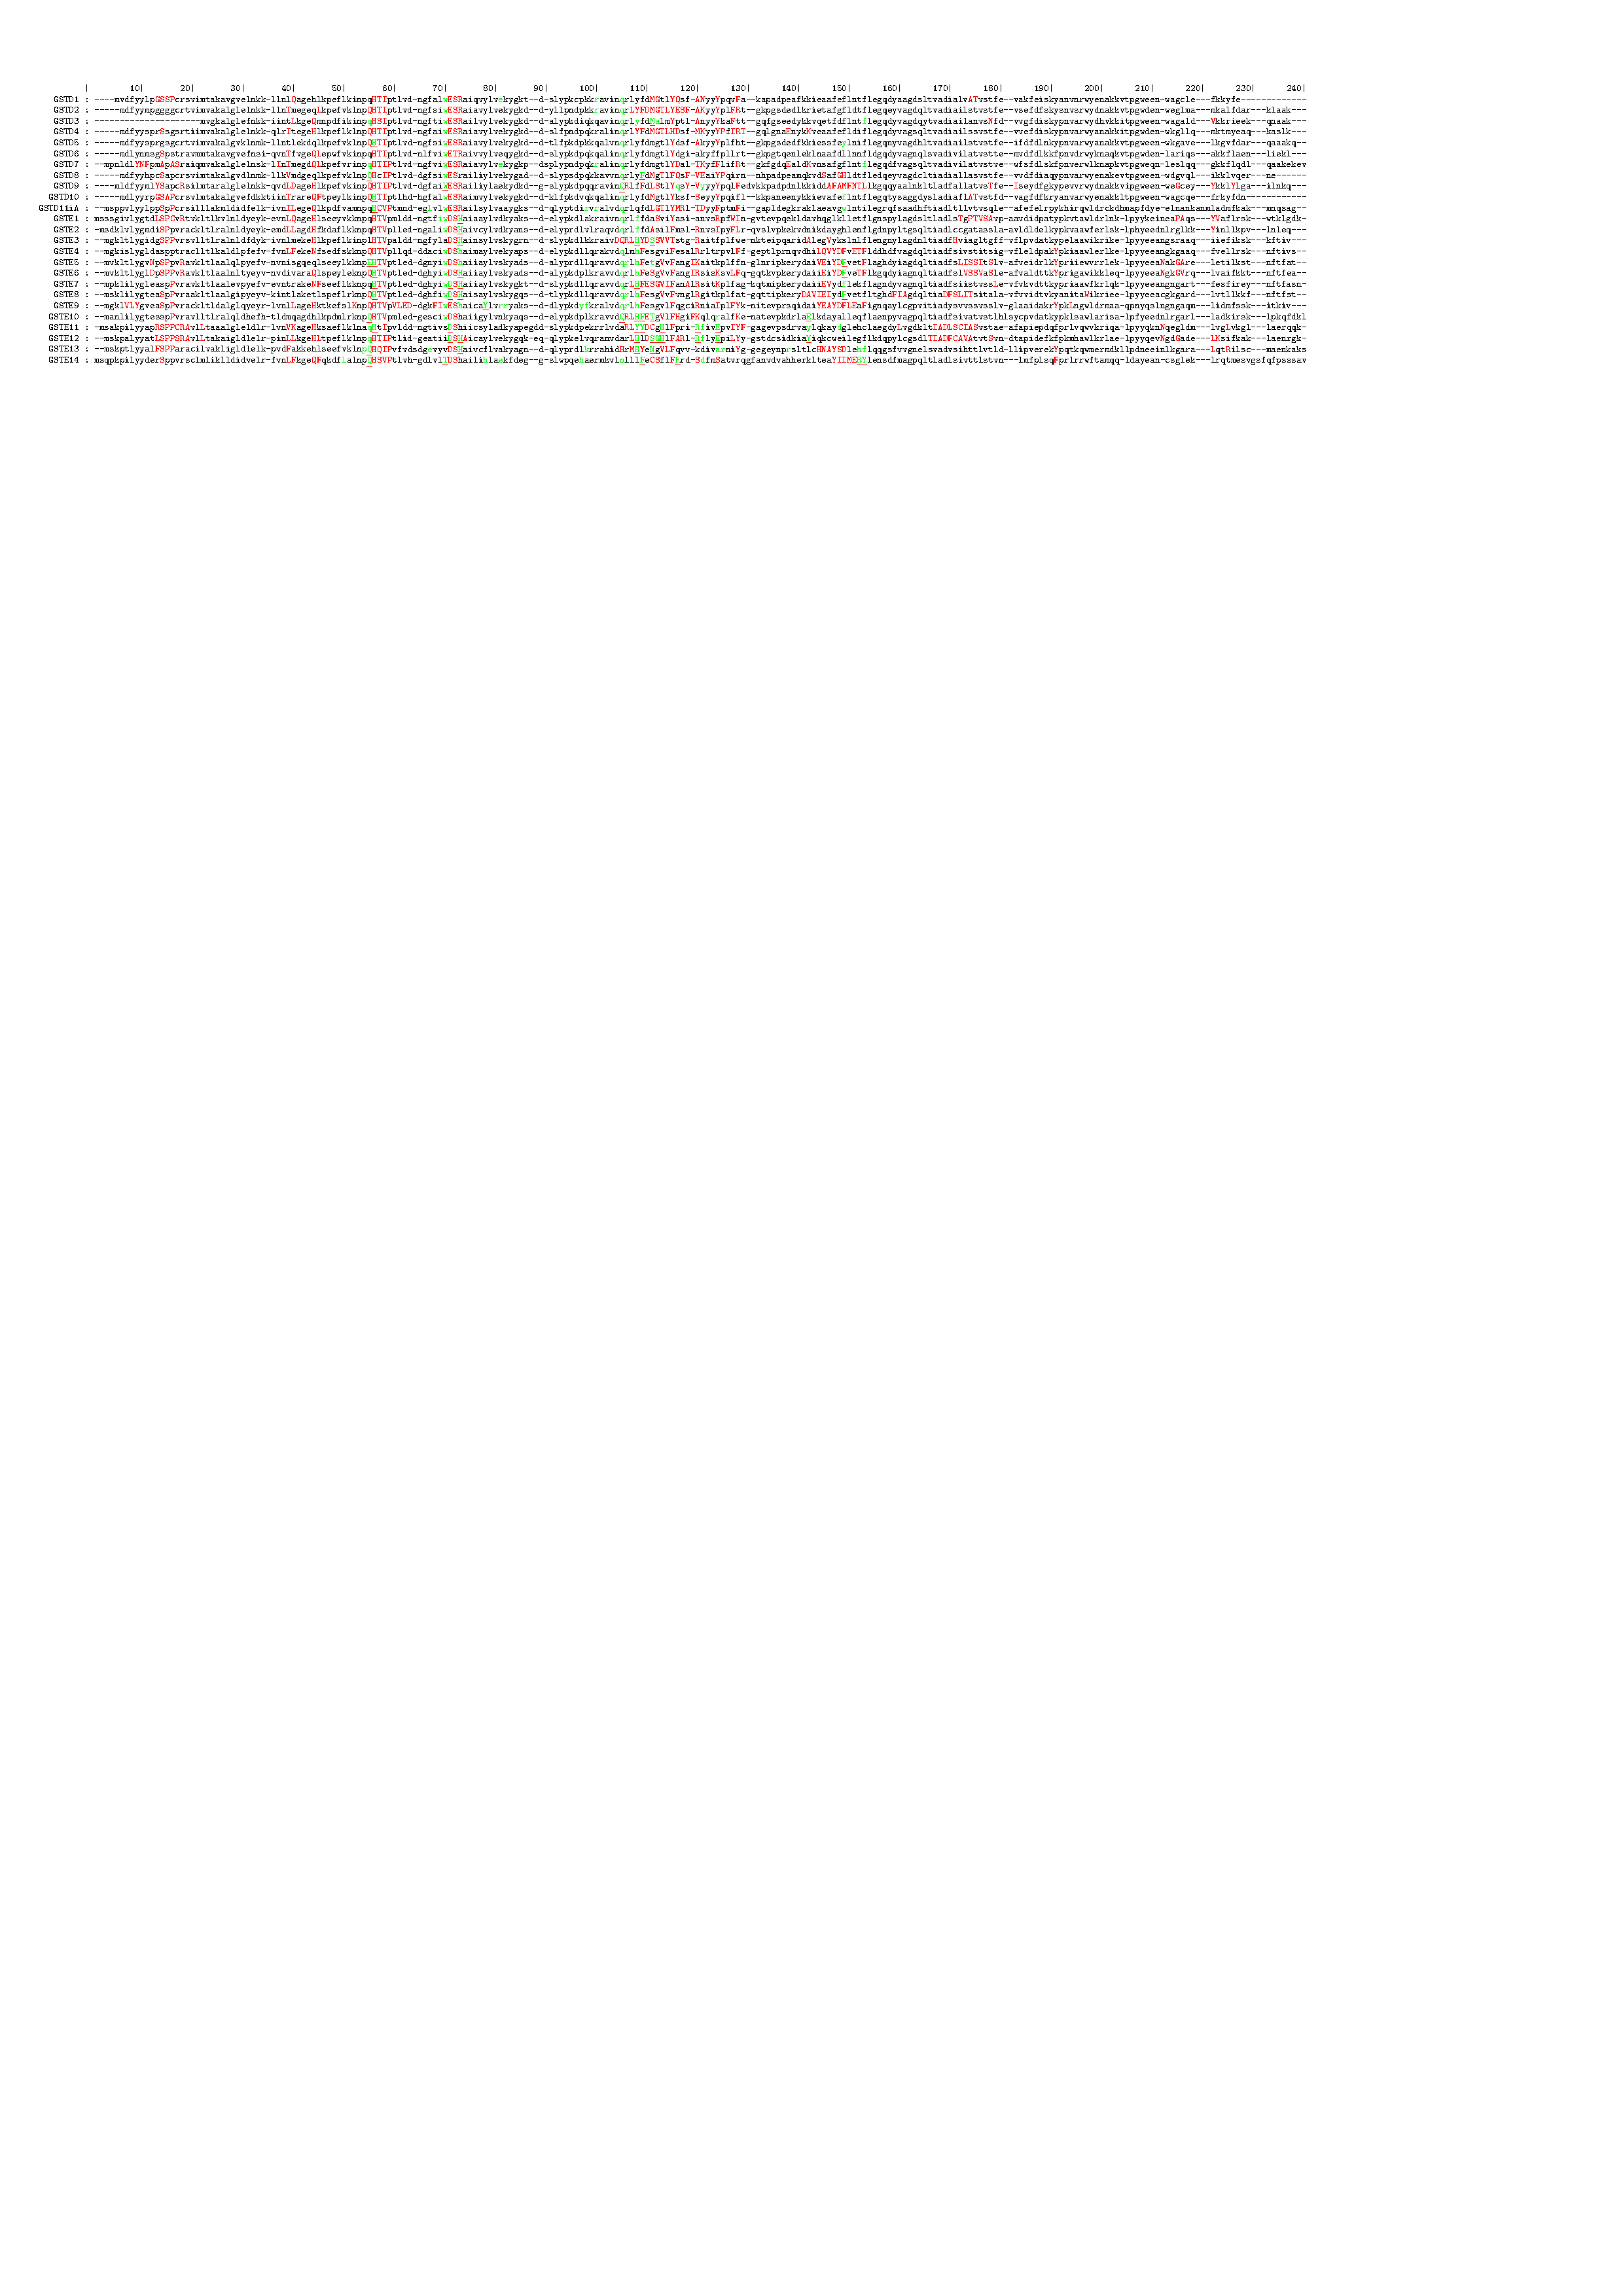
\includegraphics[width = .80\linewidth]{figures/MSA_matrix.pdf}\\[.5cm] % MSA + AF + AFi
	\textbf{B}\\
	\center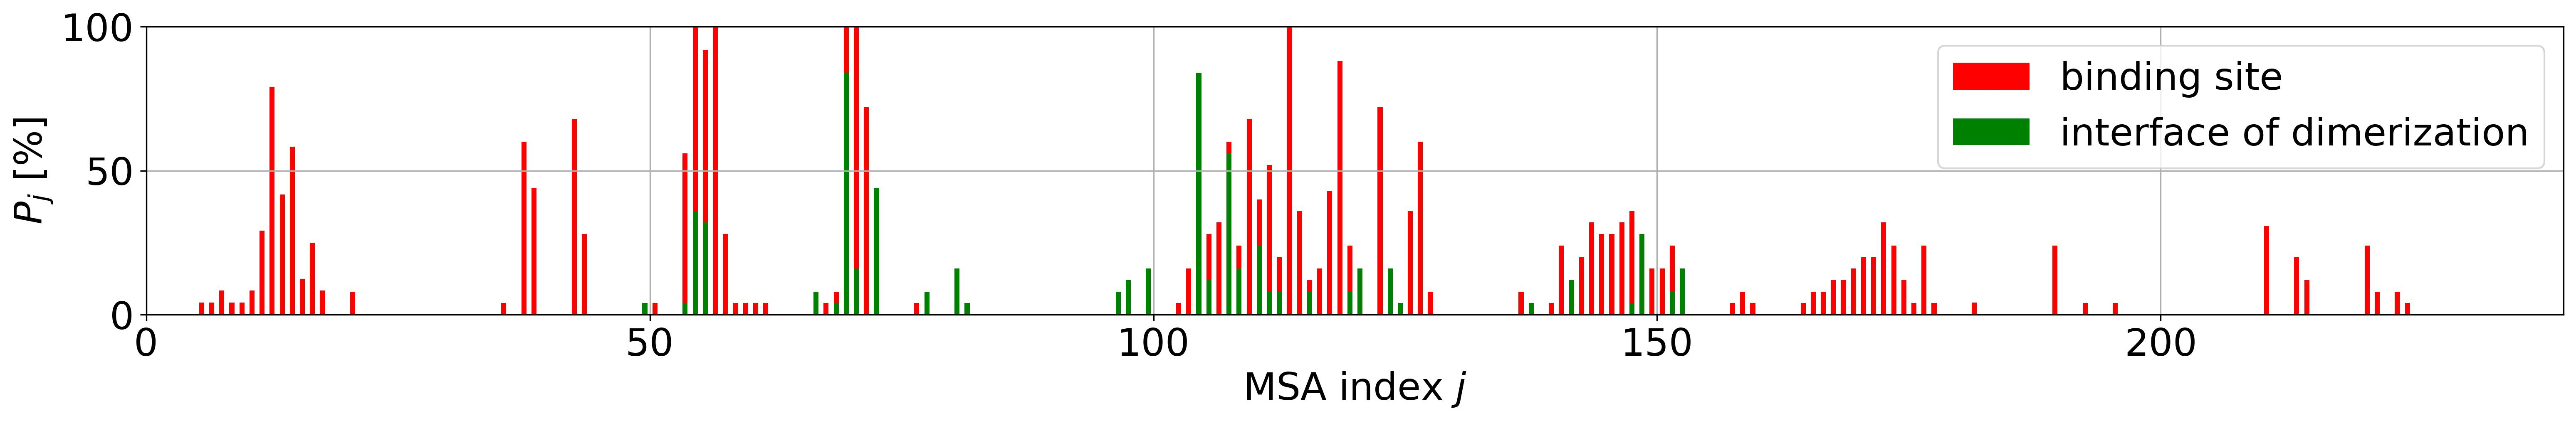
\includegraphics[height = 2.75cm]{figures/MSA_Proba.jpg} % BS & DI proba :
	\caption{Indentification of residues in the binding site and of the interface of dimerization}
\end{figure}

\newpage
\section{Dynamics from Normal Modes}
\noindent As explained in the introduction, this present work not only cares about the informations that have been extracted from the static predictions of the AlphaFold and AlphaFill programs but also about the dynamics of the dimers. In this section we will present the next step of our methodology with the Anisotropic Network Model, starting with the parametrization.

\subsection{Parametrization}
\noindent The parametrization step is needed to make sure that the predictions of the model are physically relevant. From the amino-acid's center of mass, it is very simple to compute the mass-weighted Hessian (see eq. \ref{mass-weighted hessian matrix}). As presented before, a first step is to make sure that the cut-off $R_c$ is such that the eigenvalues of the Hessian are non-null. Taking the exemple of the GSTD1, we computed $\tilde{\omega}_k^2 (R_c)$ for the modes $5$, $6$, $7$ and $8$. 

\begin{figure}[h!]
	\label{Rc param}
	\begin{minipage}{.48\linewidth}
		\textbf{A}\\
		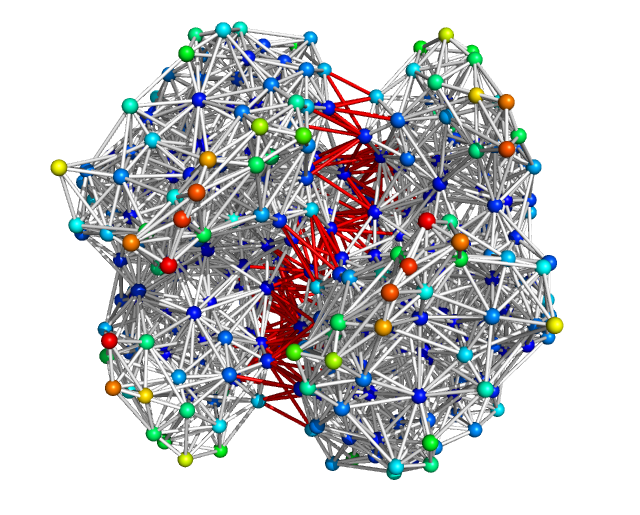
\includegraphics[width = .99\linewidth]{figures/GSTD1_ElasticNetwork.png}
	\end{minipage}	
	\begin{minipage}{.48\linewidth}
		\textbf{B}\\
		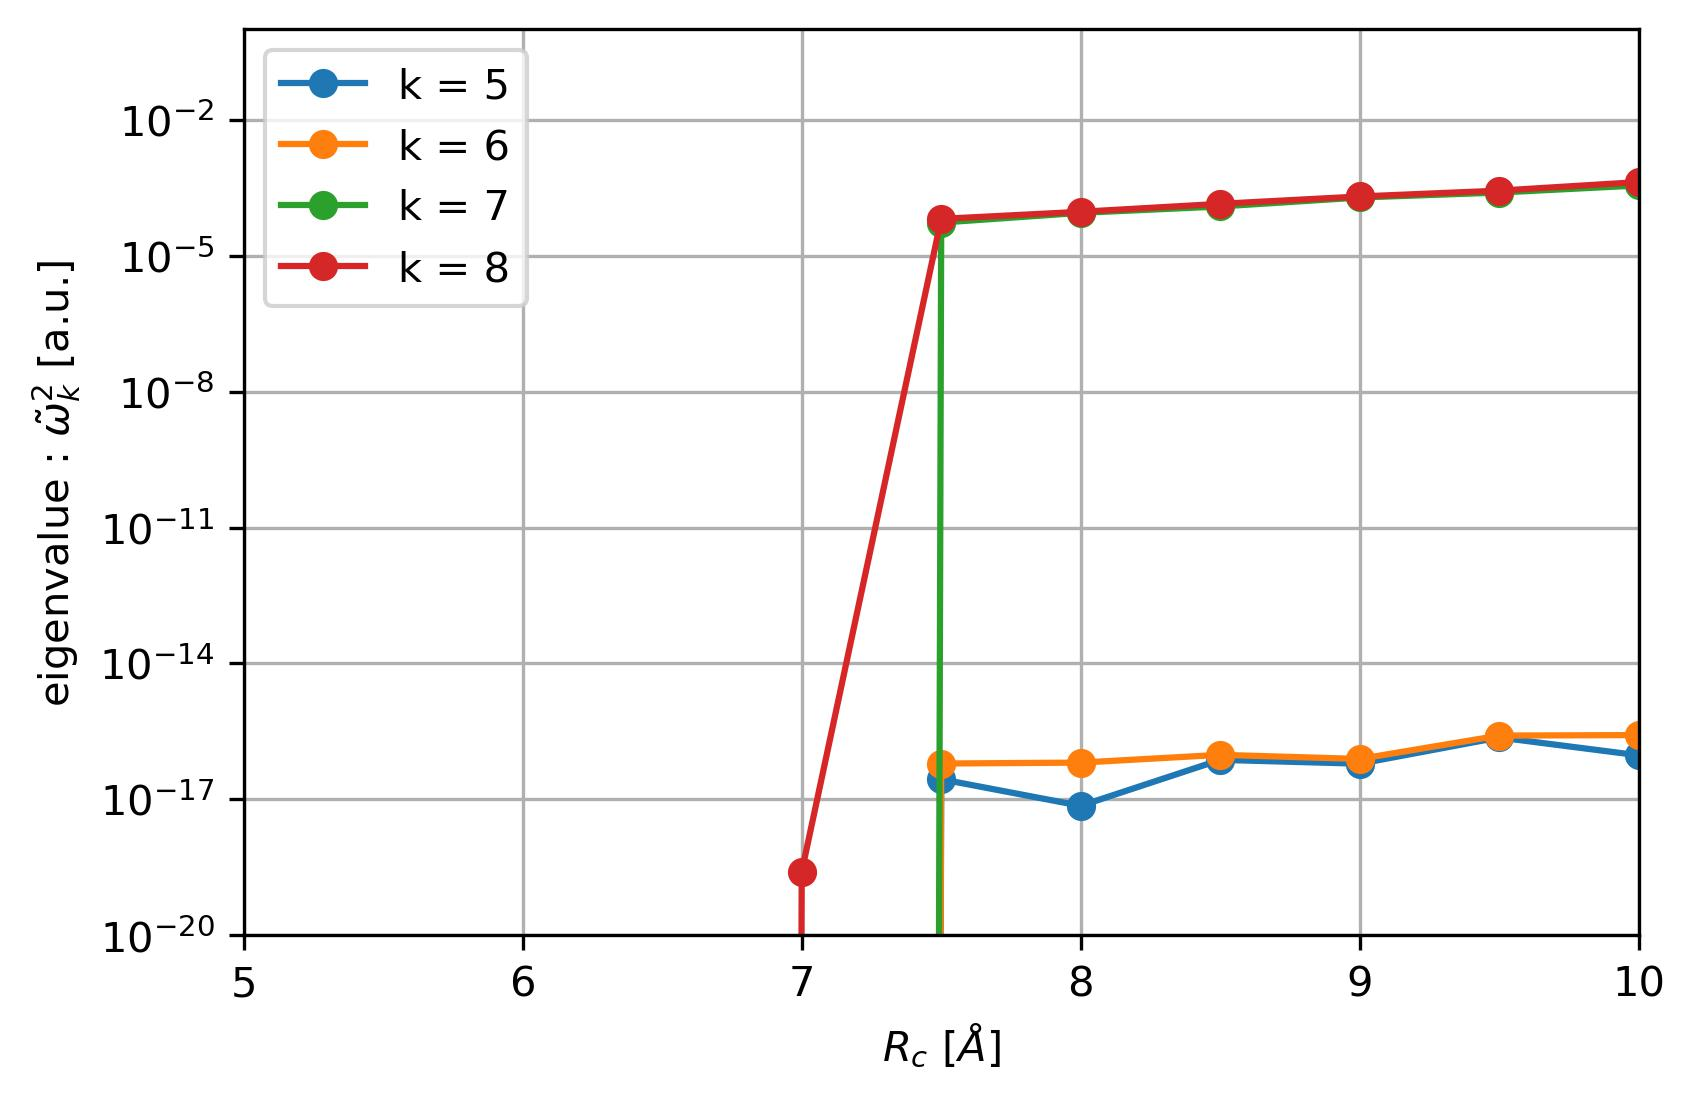
\includegraphics[width = .99\linewidth]{figures/GSTD1_ANM-COM_Rc_param.jpg}\\[.5cm]
	\end{minipage}	
	\caption{Coarse grained representation \& cut-off parametrisation of GSTD1 structure}	
\end{figure}

\noindent In the figure \ref{Rc param}, it is clearly visible that for $R_c = 7.5\AA$, the eigenvalues for $k \ge 6$ are no longer nulls. It is then convenient to use this value of cut-off for this structure. Note that later, such computations will be performed for all 25 structures in order to have a correct representation of the structures' topology. Those eigenvalues are computed for $\gamma = 1$ kcal.mol$^{-1}$.\AA$^{-2}$, but as we have seen before, $\tilde{\omega}_k^2 \propto \gamma$. It is now time to compute the thermal B-factors to be able to compute the optimal $\gamma$ value.

\subsection{Predictions}
\begin{figure}[h!]
	\label{ANM-COM D1}
	\begin{minipage}{.68\linewidth}
		\textbf{A}\\
		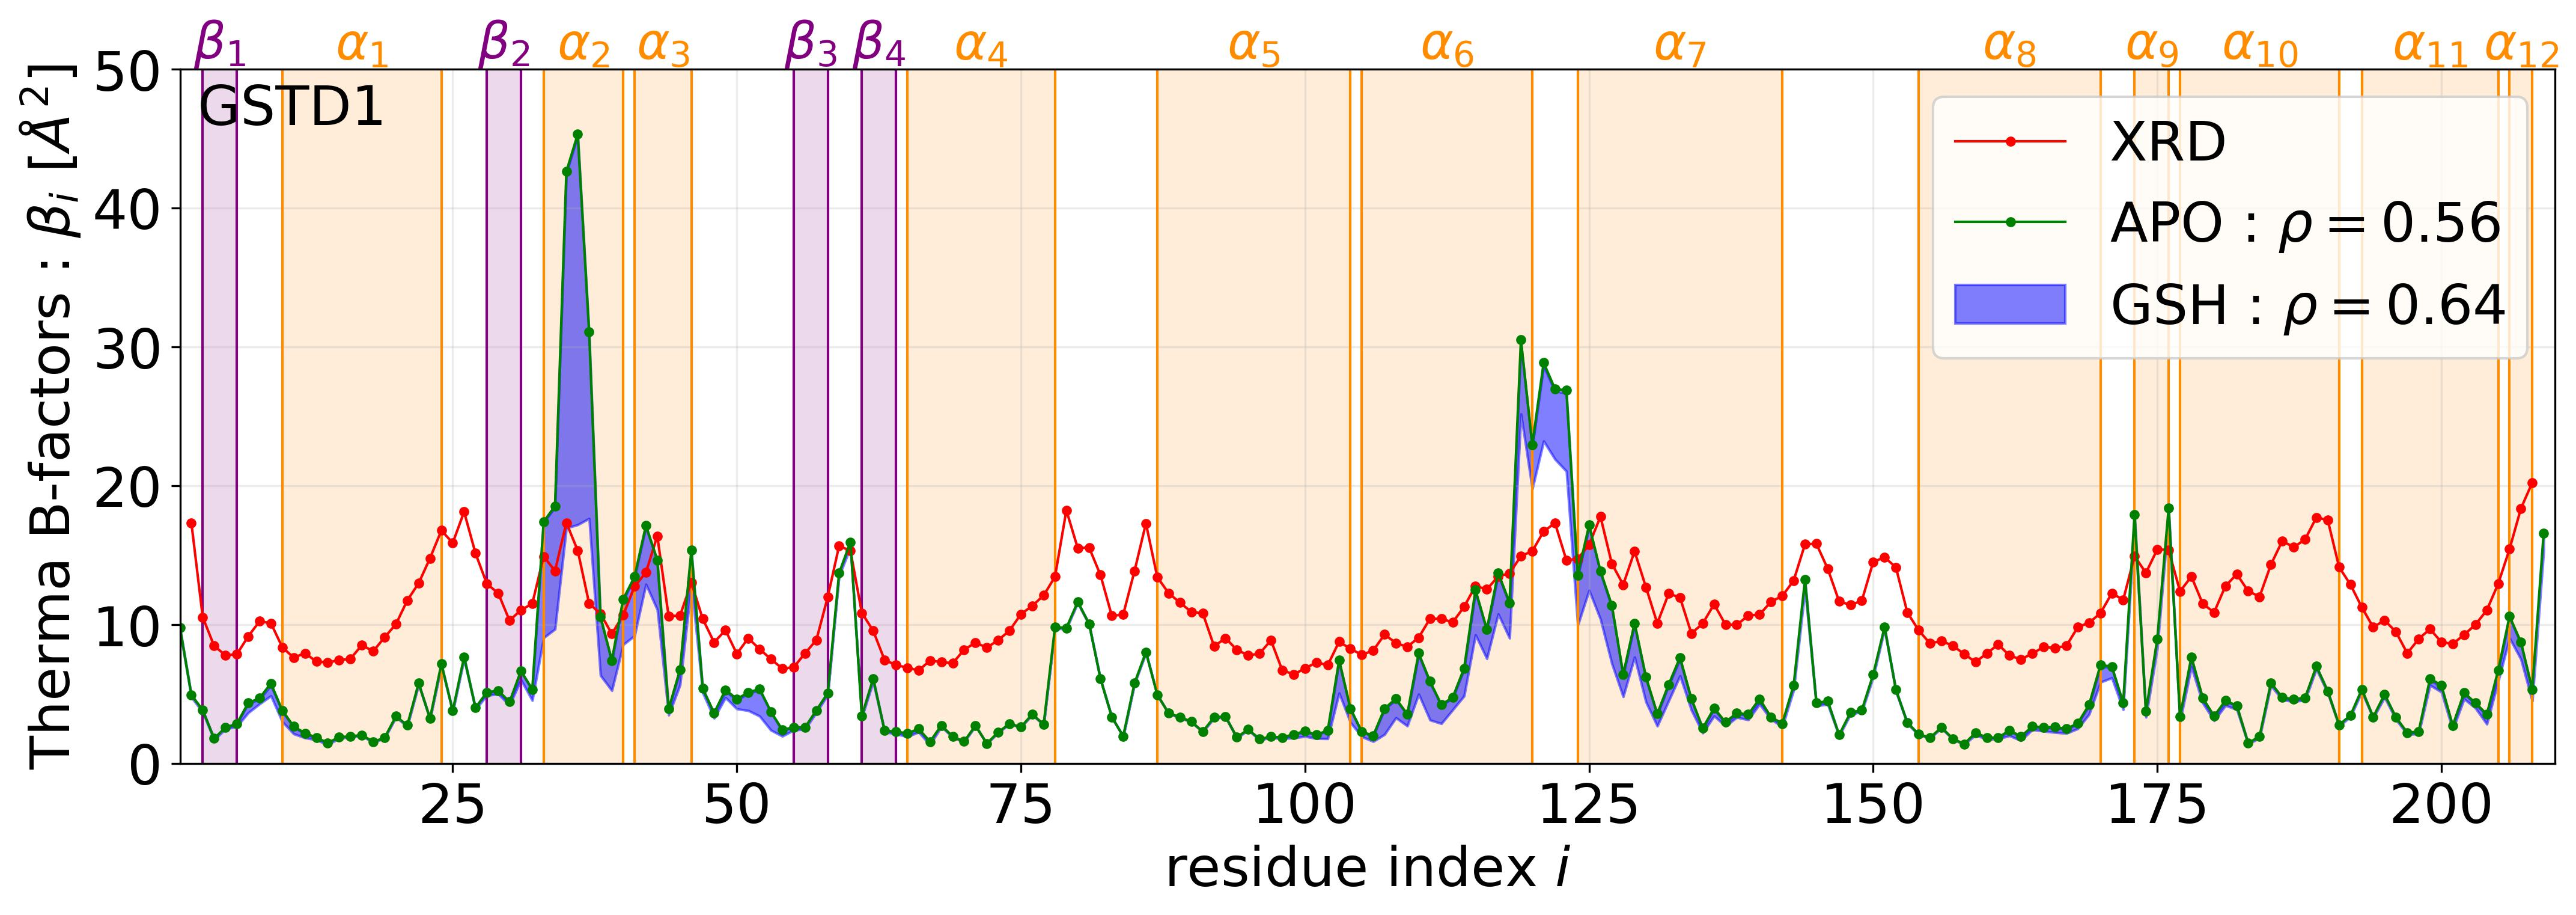
\includegraphics[height = 4cm]{figures/GSTD1+GSH_ANM-COM_Bfactors.jpg}
	\end{minipage}
	\begin{minipage}{.30\linewidth}
		\textbf{B}\\
		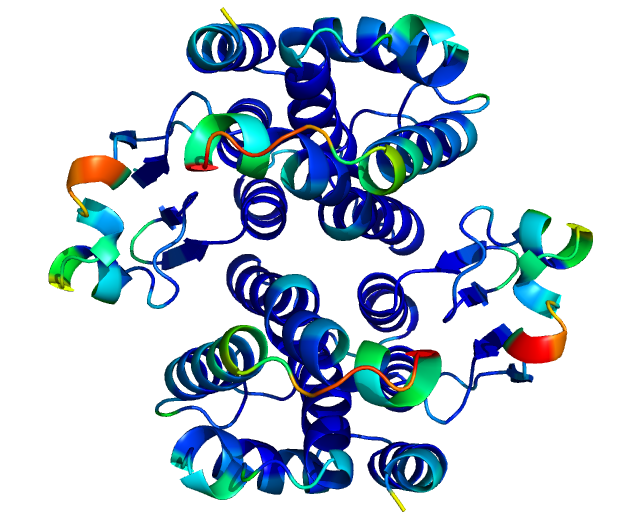
\includegraphics[height = 4cm]{figures/GSTD1_ANM-COM_Bfactors_structure.png}
	\end{minipage}
	\caption{Thermal B-factors predicted from ANM-COM and comparisions with XRD measurments}
\end{figure}

\noindent The GSTD1 structure already have been studied and a X-ray diffraction based measurment of the Thermal B-factors have been done. This curve is represented in red in the figure (\ref{ANM-COM D1}). The predictions of the ANM-COM are done first taking $R_c = 7.5$\AA ~and $\gamma = 1$kcal.mol$^{-1}$.\AA$^{-2}$, then using least squared methods to fit the predictions on the measurments, one can compute a $\gamma$ value of $14$kcal.mol$^{-1}$.\AA$^{-2}$. Eventually, it is possible to add $6$ nodes that corresponds to the amino-acids of the GSHs predicted from AlphaFill. In the case of the GSTD1, the program gives $40$ different positions. We computed the thermal B-factors for those $40$ structures (protein + ligands) and plotted the range of B-factors predicted in blue in the figure (\ref{ANM-COM D1}). From these results, there is several remarks to be done. First in the APO configuration, one can clearly see that the position of the predicted spikes matches the position of the XRD measurments, even though their relative amplitude doesn't seems to be perfect. The computation of the pearson correlation gives $56\%$. Then, taking into account the GSHs, it appears that in the regions where the ANM gives the highest predicted B-factors, the ligands introduce a bigger rigidity and reduces the predictions in the regions of index $33-52$ and $103-138$. The computed pearson correlation for the GSH was achieved taking for each residue the minimal value of B-factors within the range of $40$ predictions and gives an increase of $8\%$ comared to the APO configuration. It is also possible to look at the conservation of the residues in this range the same way we did in the previous section. Let us for instances consider the residue $34$. Projected on the MSA matrix, this gives an index of $39$ which gives the following histogram.
\begin{figure}[h!]
	\label{j=39}
	\begin{minipage}{.48\linewidth}
		For this specific index, the GSTs usually have either Leucines or Tyrosines amino-acids with a high probability or Isoleucine, Phenylalanine, Methionine or Valine with much smaller probability. All those residues have hydrophobic side chains and the main difference that can be done is the presence or abscence of aromatic rings in the amino-acid's side chain.
	\end{minipage}
	\begin{minipage}{.48\linewidth}
		\centering
		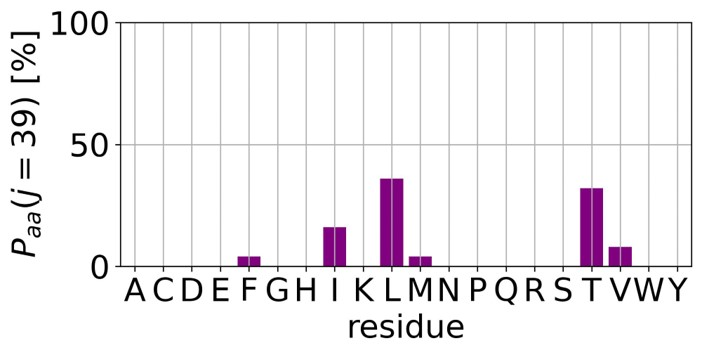
\includegraphics[height = 4cm]{figures/amino-acid_conservation_j=39.jpg}
	\end{minipage}	
	\caption{Amin-acid conservation for the 39$^{\text{th}}$ residue of the MSA matrix}
\end{figure}

\noindent So far, we have seen a methodology that allows, starting from a protein sequence to determine the associated structure and flexibility using ANM. It is now possible to extend this methodology to the set of 25 GSTs. The parameter $\gamma$ is set to be $14$ kcal.mol$^{-1}$.\AA$^{-2}$ and the $R_c$ cut-off will be systematically computed for each structure. Eventually, using a projection on the MSA matrix, it is possible to build the following representation.
\begin{figure}[h!]
	\label{ANM-COM + MSA}
	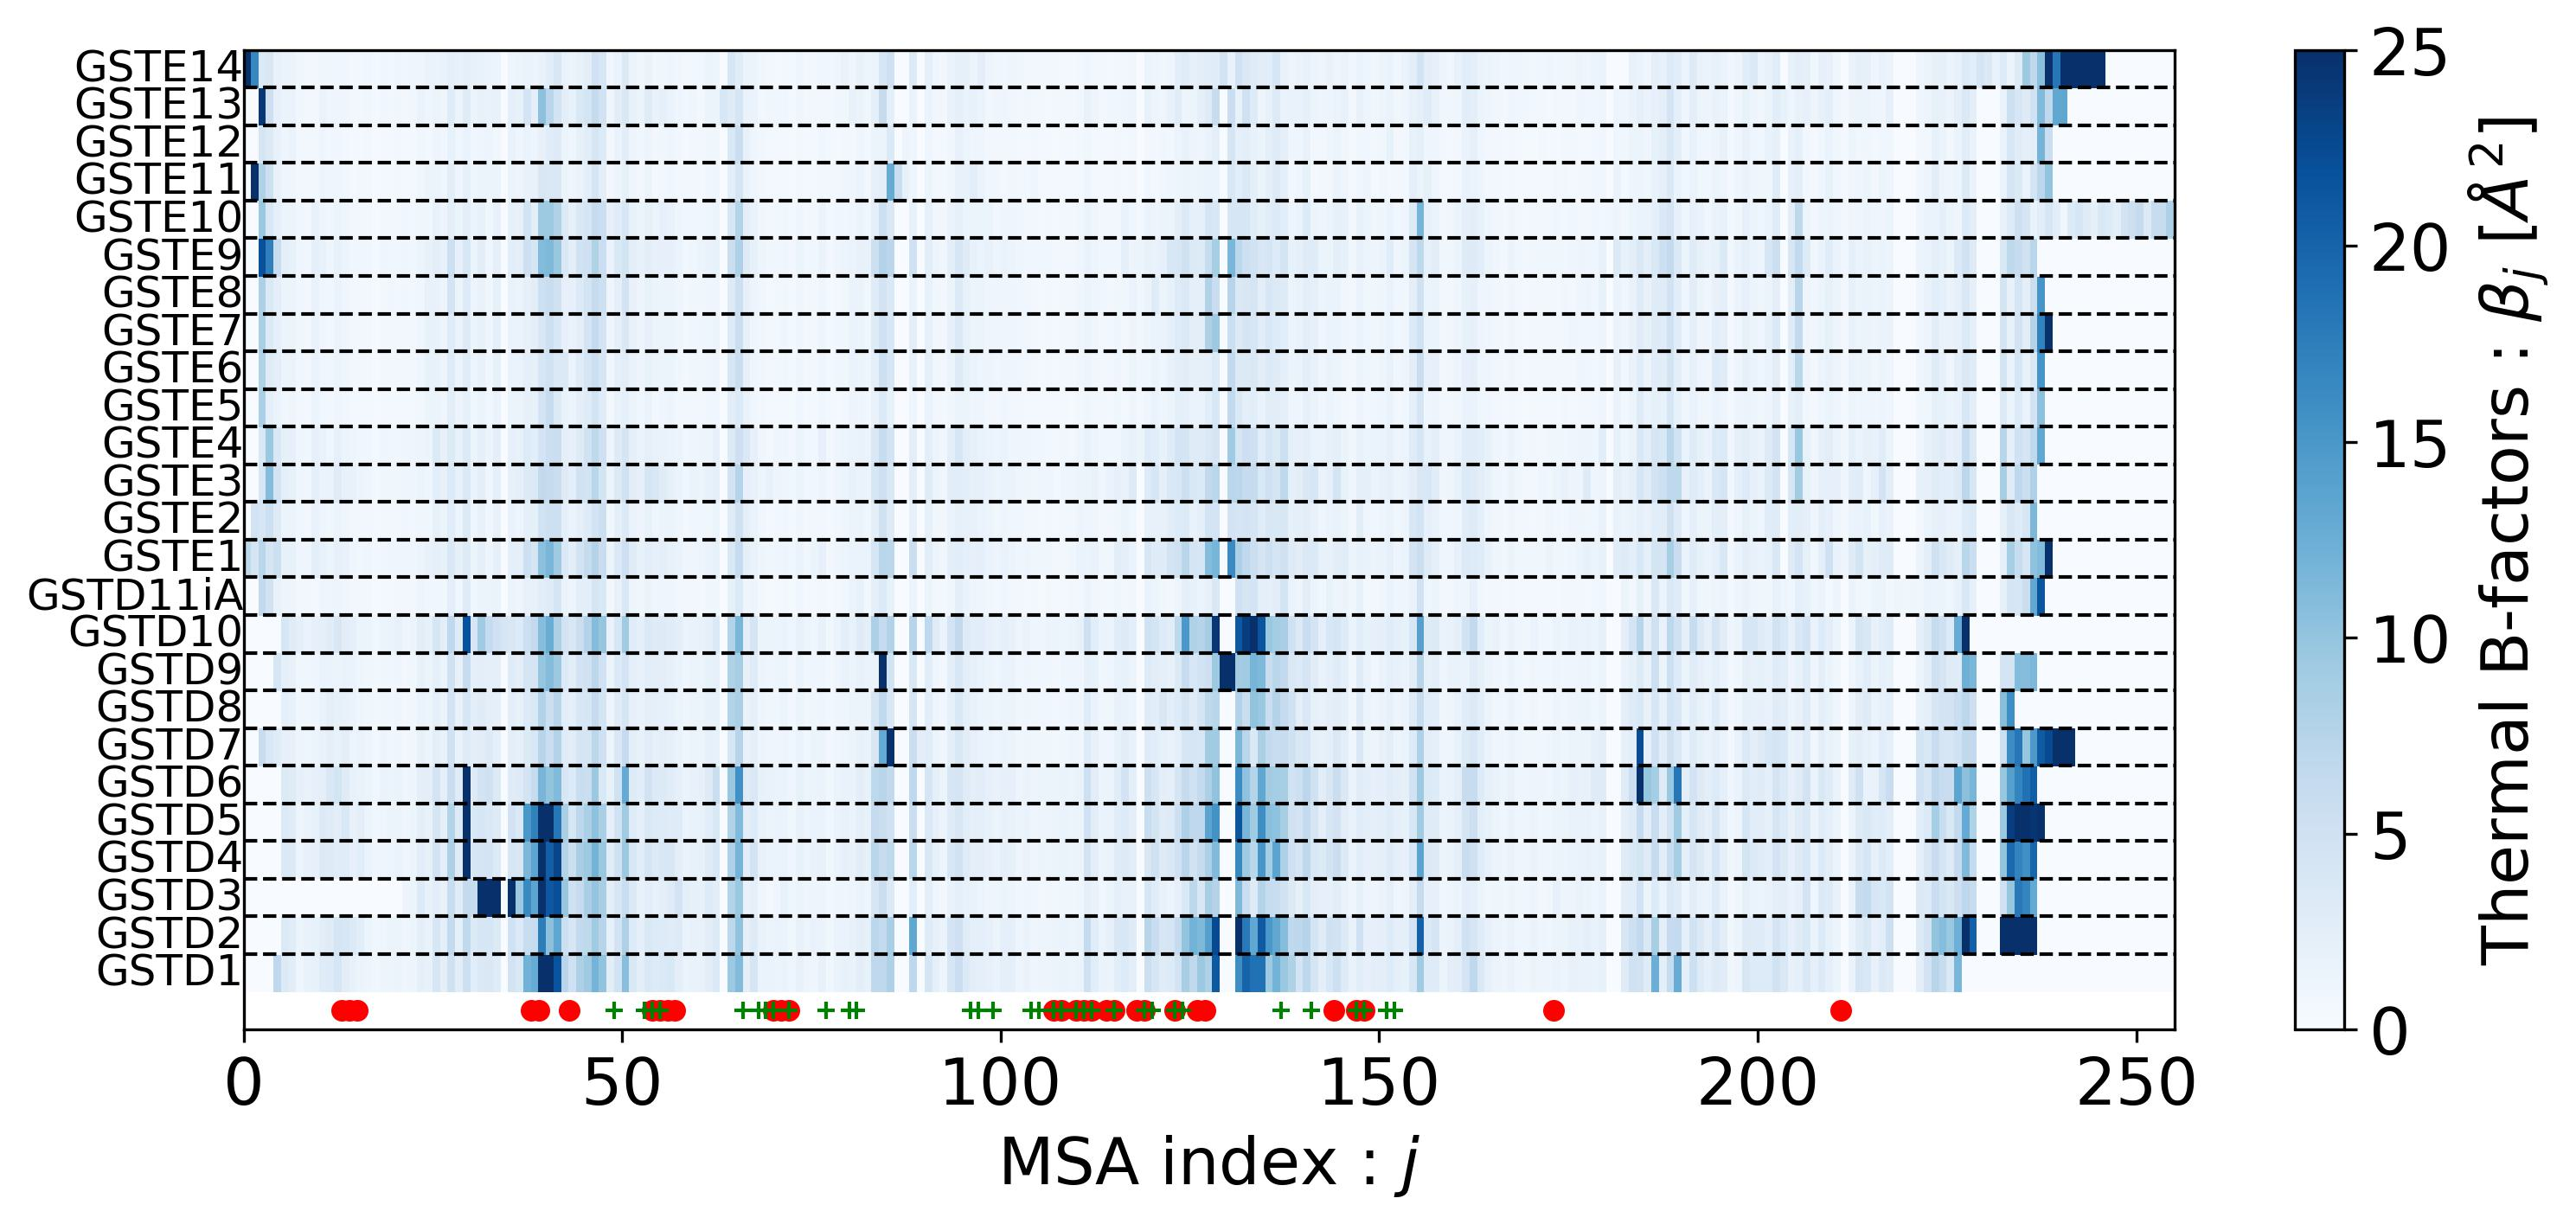
\includegraphics[width = .99\linewidth]{figures/ANM-COM_MSA_rep.jpg}
	\caption{ANM-COM prediction for the thermal B-factors of the 25 GSTs considered}
\end{figure}
\section{Dynamics from Molecular Dynamics}

\section{Comparison between Structures}